\documentclass[9pt, addpoints]{exam}

\usepackage[spanish]{babel}
\usepackage[utf8]{inputenc}
\usepackage[dvips]{graphicx}
\usepackage{amsmath}
\usepackage{amsfonts}
\usepackage{amssymb}
\usepackage{pifont}
\usepackage{multicol}
%\usepackage{psfrag}
\usepackage{color}
\usepackage{latexsym}
\usepackage{epsfig}
%\usepackage{pstricks}
%\usepackage[T1]{fontenc}
\usepackage{tikz}

% Language selection 
\newif\ifspanish
\spanishtrue % For the spanish version
\spanishfalse % For the english version

% Opción para las soluciones
\printanswers

\def\dunodcero{\begin{array}{c} D=1 \\ \gtrless \\ D=0 \end{array}}
\def\dceroduno{\begin{array}{c} D=0 \\ \gtrless \\ D=1 \end{array}}
\newcommand{\pfa}{P_{\text{FA}}} 
\newcommand{\pmis}{P_{\text{M}}} 
\newcommand{\pdet}{P_{\text{D}}} 
\newcommand{\EE}{\mathbb{E}} 

\ifspanish
\newcommand{\ej}{Ejercicio }
\else
\newcommand{\ej}{Exercise }
\fi

\hyphenation{im-pres-cin-di-ble}

\setlength{\textheight}{23cm} \setlength{\textwidth}{15cm}
\setlength{\marginparsep}{2mm} \setlength{\marginparwidth}{2cm}

\spanishdecimal{.}
\pointsinmargin
\marginpointname{\%}
\pagestyle{head}

%%%%%%%%%%
\ifspanish
\header{Procesos Estocásticos}{Problemas}{Curso Académico 2019/2020}
\else
\header{Stochastic Processes}{Problems}{Academic Year 2019/2020}
\fi

\headrule

\ifspanish
\title{{\bf Procesos Estocásticos: Problemas}}
\else
\title{{\bf Stochastic Processes: Problems}}
\fi


%%%%%%%%%%%%%%%%
\begin{document}

\maketitle

\ifspanish

%\begin{center}
%  \fbox{\fbox{\parbox{6in}{
%  Los problemas y ejercicios que se incluyen pertenecen en su mayoría a exámenes de asignaturas relacionadas con Procesos Estocásticos. 
%  }}}
%\end{center}
%\begin{center}
%  \fbox{\fbox{\parbox{6in}{\centering Notación: \begin{itemize}
% \item Decisor ML: Decisor de máxima verosimilitud [$\phi_{\rm ML}(\mathbf x)$].
%   \end{itemize}
%  }}}
%\end{center}

\else

%\begin{center}
%  \fbox{\fbox{\parbox{6in}{
%  Most of the problems and exercises of this collection have been taken from previous years exams on subjects related to Stochastic Processes.
%  }}}
%\end{center}
%\begin{center}
%  \fbox{\fbox{\parbox{6in}{\centering Notation: \begin{itemize}
% \item ML decider: Maximum likelihood decider [$\phi_{\rm ML}(\mathbf x)$].
%  \item MAP decider: Maximum {\em a posteriori} decider [$\phi_{\rm MAP}(\mathbf x)$].
%   \end{itemize}
%  }}}
%\end{center}

\fi

%%%%%%%%%%%%%%%%%%%%%%%%%%
\section{Markov Processes}
%%%%%%%%%%%%%%%%%%%%%%%%%%

%%%%%%%%%%%%%%%%%
\begin{questions}

%%%%%%%%
\qformat{\textbf{\ej MP\thequestion ~~ (Markov Chain)} ~~ \linefill}
\question
\ifspanish

TBD

\else

Let ${X_k, k \ge 0}$ be a Markov chain with state space ${\cal Z} = \{0, 1\}$ and transition probabilities $P\{X_k=1 | X_{k-1}=0\} = 0.8$ and $P\{X_k=0 | X_{k-1}=1\} = 0.4$.

\begin{parts}
\part Draw the corresponding transition graph
\part Assume that the initial state is  $X_0 = 1$. Compute $P\{X_2=1\}$
\part Compute the stationary distribution.
\end{parts}

\begin{solution}
\begin{parts}
\part The transition matrix is 
$$
{\bf P} = \begin{pmatrix}
0.2 & 0.8 \\
0.4 & 0.6
\end{pmatrix}
$$
and, thus, the transition graph is

{\centering
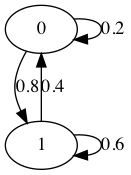
\includegraphics[scale=0.3]{db/figs/MPbinary.png}}

\part 
$$
P\{X_2=1\} = 
    \begin{pmatrix} 0 & 1 \end{pmatrix}
    {\bf P}^\intercal{\bf P}^\intercal
    \begin{pmatrix} 0 \\ 1 \end{pmatrix} 
    = 0.68
$$ 
\part The stationary distribution is the solution of
$$
{\bf P}^\intercal \boldsymbol{\pi} = \boldsymbol{\pi}
$$ 
with $(1, 1) \boldsymbol{\pi} = 1$, that is:
$$
0.2 \pi_0 + 0.4 \pi_1 = \pi_0
$$
and taking $\pi_1 = 1-\pi_0$, we get
$$
0.4 (1-\pi_0)  = 0.8 \pi_0
$$
so that $\pi_0 = \frac13$  and
$$
(\pi_0, \pi_1) = \left(\dfrac13, \dfrac23\right)
$$
\end{parts}
\end{solution}

\fi

%%%%%%%%
\qformat{\textbf{\ej MP\thequestion ~~ (Markov Process)} ~~ \linefill}
\question
\ifspanish

Un videojuego consta de $N$ niveles consecutivos, $0, 1, ..., N-1$. El jugador empieza en el nivel 0. Si un jugador pasa el nivel $i$, entra en el nivel $i+1$, si no, vuelve al nivel 0. Se sabe que todas las fases tienen la misma dificultad, por lo que si jugador está en el nivel $i$, alcanza el nivel $i+1$ con probabilidad $q$, y regresa a 0 con probabilidad $1-q$.

Cuando el jugador alcanza la etapa $N-1$, obtiene una medalla, vuelve al nivel 0 y el juego continúa.

Sea $X_k$ el proceso estocástico que representa la secuencia de niveles durante un juego, tal que $X_k=i$ significa que el jugador estaba en el nivel $i$ en el momento $k$. El juego comienza en $X_0=0$.
\begin{parts}
\part Formule el problema como un proceso de Markov estacionario y dibuje el gráfico de transición para $N = 6$.
\part Asumiendo $N \ge 2$, calcule $P\{X_2=1\}$.
\part Suponiendo $N \ge 2$, determine la probabilidad de obtener una medalla exactamente en el tiempo $k$, es decir $P\{X_k=N-1\}$, para $k=0,1, \ldots, N$.
\part Para $N=2$, determine la distribución estacionaria.
\part Para $N=\infty$, determine la distribución estacionaria

\end{parts}

\begin{solution}
\begin{parts}
\part El grafo de transición se muestra en la figura para $q=0.1$.

{\centering
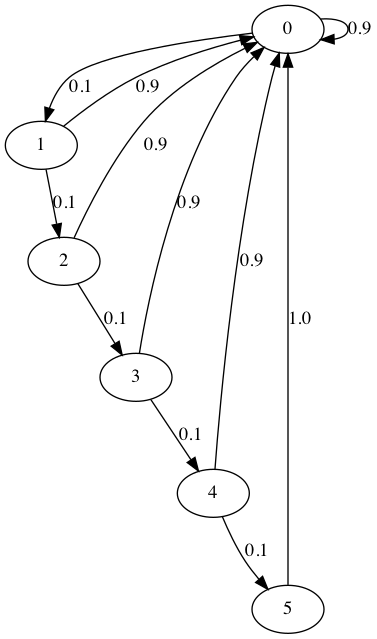
\includegraphics[scale=0.3]{db/figs/SPES_202106_markov_chain.png}}

\part 
\begin{align*}
P\{X_2=1\} = q P\{X_1=0\} = q (1-q) P\{X_0=0\} = q (1-q) 
\end{align*}

\part La probabilidad de obtener una medalla en el momento $k$ es $Q_k=P\{X_k=N-1\}$. Daddo que se requieren al menos $N-1$ pasos para alcanzar el nivel $N-1$, resulta
\begin{align*}
Q_k = 0,     \qquad \text{ for } k=0, \ldots, N-2
\end{align*}

Alcanzar el nivel $N-1$ en el momento $k=N-1$ is posible solamente si el jugador no falla en ninguna ocasión, de modo que
\begin{align*}
Q_{N-1} = q^{N-1}
\end{align*}

Alcanzar el nivel $N-1$ en $k=N$ es posible solamente si el jugador falla en el instante $0$ únicamente, de modo que
\begin{align*}
Q_{N} = (1-q) q^{N-1}
\end{align*}

\part Dado que
\begin{align*}
\pi_1 = q \pi_0
\end{align*}
y $\pi_0 + \pi_1 = 1$, resulta
\begin{align*}
\pi_1 = \frac{q}{1+q}
\end{align*}

\part Para $i>0$, se tiene que
\begin{align*}
\pi_i = q \pi_{i-1} = q^2 \pi_{i-2} = \ldots = q^i \pi_0
\end{align*}
y, para $i=0$,
\begin{align*}
\pi_0 = \sum_{i=0}^\infty (1-q) \pi_i 
       = (1-q) \sum_{i=0}^\infty \pi_i 
       = 1-q
\end{align*}
de modo que
\begin{align*}
\pi_i = (1-q) q^i
\end{align*}

\end{parts}
\end{solution}

\else

A video game consists of $N$ consecutive levels, $0, 1, ..., N-1$. The player starts at level 0. If a player passes level $i$, she enters level $i+1$, if not, she returns back to level 0. It is known that all phases have the same difficulty, so, if a player is at level $i$, she reaches level $i+1$ with probability $q$, and returns back to 0 with probability $1-q$. 

When the player reaches stage $N-1$, she gets a medal, returns to level 0 and the game continues.

Let $X_k$ be the stochastic process that represents the sequence of levels during a game, such that $X_k=i$ means that the player was at level $i$ at time $k$. The game begins at $X_0=0$.
\begin{parts}
\part Formulate the problem as a stationary Markov process, and draw the transition graph for $N = 6$.
\part Assuming $N \ge 2$, compute $P\{X_2=1\}$.
\part Assuming $N \ge 2$, determine the probability of obtaining a medal exactly at time $k$, that is $P\{X_k=N-1\}$, for $k=0,1, \ldots, N$.
\part For $N=2$, determine the stationary distribution.
\part For $N=\infty$, determine the stationary distribution

\end{parts}

\begin{solution}
\begin{parts}
\part The transition graph is shown in the figure for $q=0.1$.

{\centering
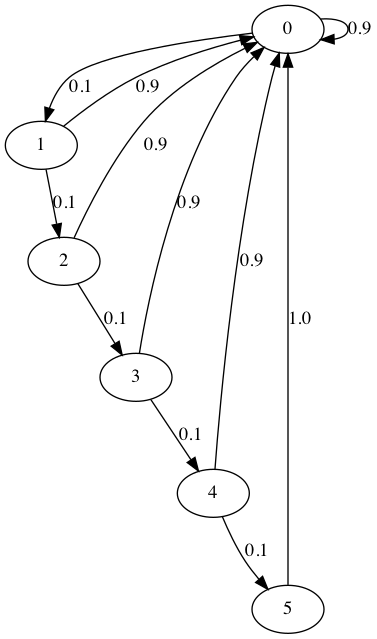
\includegraphics[scale=0.3]{db/figs/SPES_202106_markov_chain.png}}

\part 
\begin{align*}
P\{X_2=1\} = q P\{X_1=0\} = q (1-q) P\{X_0=0\} = q (1-q) 
\end{align*}

\part The probability of obtaining a medal at time $k$ is $Q_k=P\{X_k=N-1\}$. Since at least $N-1$ steps are required to reach level $N-1$, we have
\begin{align*}
Q_k = 0,     \qquad \text{ for } k=0, \ldots, N-2
\end{align*}

Reaching level $N-1$ at time $k=N-1$ is possible only if the player does not fail at any time, so that
\begin{align*}
Q_{N-1} = q^{N-1}
\end{align*}

Reaching level $N-1$ at time $k=N$ is possible only if the player fails at time $0$ only, so that.
\begin{align*}
Q_{N} = (1-q) q^{N-1}
\end{align*}

\part Since
\begin{align*}
\pi_1 = q \pi_0
\end{align*}
and $\pi_0 + \pi_1 = 1$, we have
\begin{align*}
\pi_1 = \frac{q}{1+q}
\end{align*}

\part For $i>0$, we have
\begin{align*}
\pi_i = q \pi_{i-1} = q^2 \pi_{i-2} = \ldots = q^i \pi_0
\end{align*}
and, for $i=0$,
\begin{align*}
\pi_0 = \sum_{i=0}^\infty (1-q) \pi_i 
       = (1-q) \sum_{i=0}^\infty \pi_i 
       = 1-q
\end{align*}
so that
\begin{align*}
\pi_i = (1-q) q^i
\end{align*}

\end{parts}
\end{solution}


\fi

\end{questions}

%%%%%%%%%%%%%%%%%%%%%%%%%%%%%%%
\section{Stationary Processes}
%%%%%%%%%%%%%%%%%%%%%%%%%%%%%%%

%%%%%%%%%%%%%%%%%
\begin{questions}

%%%%%%%%
\qformat{\textbf{\ej SP\thequestion ~~ (Autocorrelation, Power Spectrum)} ~~ \linefill}
\question
\ifspanish

TBD

\else

Let $X_n$ be i.i.d. stochastic process with probability density function
\[
p_{X}(x) = x \exp(-x), \qquad x \ge 0
\]

Assume that $X_n$ is the input to a linear system with impulse response
\[
h_n = \delta[n] + 0.5 \delta[n-1]
\]
the system output $Y_n$, is corrupted by a Gaussian i.i.d noise $E_n$ (independent of $X_n$) with mean zero and unit variance, to produce the final process
\[
Z_n =  Y_n + E_n
\]

\begin{parts}
\part Compute the autocorrelation functions $r_X[n]$ and $r_E[n]$ of $X_n$ and $E_n$, respectively.
\part Compute the autocorrelation function of $Y_n$,  $r_Y[n]$
\part Compute the autocorrelation function of $Z_n$,  $r_Z[n]$
\part Compute the power spectrum of $Z_n$, $S_Z(\omega)$..
\end{parts}

\begin{solution}
\begin{parts}
\part 
Since $X_n$ is zero-mean i.i.d, we have
\begin{align*}
r_X[n] 
	&= \EE	\{X_k X_{k+n} \} = 
       \left[
	   \begin{array}{ll}
	   \EE\{X_k^2\},            & n=0 \\
	   \EE\{X_k\}\EE\{X_{k+n}\}, & n \neq 0	
	   \end{array}
	   \right. \\
	&= \EE\{X_k^2\} \delta[n] + \EE\{X_k\}^2 (1-\delta[n])   \\
	&= \left(\EE\{X_k^2\} - \EE\{X_k\}^2\right) \delta[n] + \EE\{X_k\}^2
\end{align*}
Noting that
\begin{align*}
\EE\{X_k\}   &= \int_0^\infty x^2 \exp(-x)dx = 2  \\
\EE\{X_k^2\} &= \int_0^\infty x^3 \exp(-x)dx = 6
\end{align*}
we get
\begin{align*}
r_X[n] = 2 \delta[n] + 4
\end{align*}

Since $E_n$ is zero-mean i.i.d, we have
\begin{align*}
r_E[n] = \sigma_E^2 \delta[n] = \delta[n]
\end{align*}

\part Since
\begin{align*}
Y_n = X_n \ast h_n 
\end{align*}
we have
\begin{align*}
r_Y[n] 
	&= r_X[n] \ast h_n \ast h_{-n} \\
	&= (2 \delta[n] + 4) \ast (\delta[n] + 0.5\delta[n-1]) \ast (\delta[n] + 0.5\delta[n+1]) \\
	&= (2 \delta[n] + 4) \ast (1.25 \delta[n] + 0.5\delta[n-1] + 0.5\delta[n+1]) \\
	&= 2.5 \delta[n] + \delta[n-1] + \delta[n+1] + 9
\end{align*}

\part Since $Y_n$ and $E_n$ are independent and $E_n$ is zero-mean
\begin{align*}
r_Z[n] = r_Y[n] + r_E[n] = 3.5 \delta[n] + \delta[n-1] + \delta[n+1] + 9
\end{align*}

\part Computing the Fourier transform of the autocorrelation function, we get
\begin{align*}
S_Z(\omega) = 3.5 + 2 \cos(\omega) + 18 \pi \delta(\omega),    \qquad \omega \in [-\pi, \pi]
\end{align*}

\end{parts}
\end{solution}

\fi

%%%%%%%%
\qformat{\textbf{\ej SP\thequestion ~~ (Autocorrelation, Power Spectrum)} ~~ \linefill}
\question
% JCS

\ifspanish

El proceso estocástico $X_n$ viene dado por el par de ecuaciones
\begin{align*}
X_n &= S_n \cdot R_n \\
S_n &= W_n - \frac12 W_{n-1}
\end{align*}
donde $W_n$ es un proceso i.i.d. gausiano con media $0$ y varianza $v$, y $R_n$ es un proceso estacionario con función de autocorrelación
\begin{align*}
r_R[n] = 2^{-|n|}
\end{align*}
Los procesos $W_n$ y $R_n$ son independientes entre sí.
\begin{parts}
\part Calcule la función de autocorrelación de $W_n$, $r_W[n]$
\part Calcule y dibuje la función de autocorrelación de $S_n$, $r_S[n]$
\part Calcule y dibuje la función de autocorrelación de $X_n$, $r_X[n]$
\part Calcule el espectro de potencia del proceso $Z_n = \sum_{k=0}^\infty 2^{-k} X_{n-k}$
\end{parts}

\begin{solution}
\begin{parts}
\parte
\begin{align*}
r_W[n] = v \delta[n]
\end{align*}
\parte
\begin{align*}
r_S[n] &= \mathbb{E}\{S_k \cdot S_{k+n}\} \\
       &= \mathbb{E}\{(W_k - \frac12 W_{k-1})(W_{k+n} - \frac12 W_{k+n-1})\} \\
       &= \frac{5}{4} v \delta[n] - \frac12 v \delta[n-1] - v \frac12 \delta[n+1] \\
\end{align*}
\parte
\begin{align*}
r_X[n] &= \mathbb{E}\{X_k \cdot X_{k+n}\} \\
       &= \mathbb{E}\{S_k \cdot S_{k+n}\} \mathbb{E}\{R_k \cdot R_{k+n}\} \\
       &= r_S[n] r_R[n] \\
       &= 2^{-|n|} \cdot
          \left(\frac{5}{4} v \delta[n] - \frac12 v \delta[n-1] - v \frac12 \delta[n+1]\right) \\
       &= \frac{5}{4} v \delta[n] - \frac14 v \delta[n-1] - \frac14 v \delta[n+1])
\end{align*}
\parte
\begin{align*}
Z_n &= X_n \ast h[n]
\end{align*}
donde $h_n = 2^{-n} u[n]$. Por lo tanto
\begin{align*}
S_Z(\omega) 
     &= S_X(\omega) |H(\omega)|^2 \\
     &= \frac{v}{2} \left(\frac52 - \cos(\omega)\right) \left|\frac{1}{1-\frac12 \exp(-j\omega)}\right|^2   \\
     &= \frac{v}{2} \cdot \frac{\frac52 - \cos(\omega)}{ \left|1-\frac12 \exp(-j\omega)\right|^2}  \\
     &= v \cdot \frac{5 - 2 \cos(\omega)}{5 - 4\cos(\omega)}
\end{align*}
\end{parts}
\end{solution}

\else

The stochastic process  $X_n$ is given by the  pair of equations
\begin{align*}
X_n &= S_n \cdot R_n   \\
S_n &= W_n - \frac12 W_{n-1}
\end{align*}
where $W_n$ is a Gaussian i.i.d. process with mean $0$ and variance $v$, and $R_n$ is stationary processes with autocorrelation function
\begin{align*}
r_R[n] = 2^{-|n|} 
\end{align*}
Processes $W_n$ and $R_n$ are mutually independent.

\begin{parts}
\part Compute the autocorrelation function of $W_n$, $r_W[n]$
\part Compute and draw the autocorrelation function of $S_n$, $r_S[n]$
\part Compute and draw the autocorrelation function of $X_n$, $r_X[n]$
\part Compute the power spectrum of the process $Z_n = \sum_{k=0}^\infty 2^{-k} X_{n-k}$
\end{parts}


\begin{solution}
\begin{parts}
\part Since $W_n$ is zero-mean i.i.d, $r_W[n] = v \delta[n]$
\part 
\begin{align*}
r_S[n] &= \mathbb{E}\{S_k \cdot S_{k+n}\}   \\
       &= \mathbb{E}\{(W_k - \frac12 W_{k-1})(W_{k+n} - \frac12 W_{k+n-1})\} \\
       &= \frac{5}{4} v \delta[n] - \frac12 v \delta[n-1] - v \frac12 \delta[n+1] 
\end{align*}
\part
\begin{align*}
r_X[n] &= \mathbb{E}\{X_k \cdot X_{k+n}\}   \\
       &= \mathbb{E}\{S_k \cdot S_{k+n}\} \mathbb{E}\{R_k \cdot R_{k+n}\}  \\
       &= r_S[n] r_R[n]   \\
       &= 2^{-|n|} \cdot
          \left(\frac{5}{4} v \delta[n] - \frac12 v \delta[n-1] - v \frac12 \delta[n+1]\right) \\
       &= \frac{5}{4} v \delta[n] - \frac14 v \delta[n-1] - \frac14 v \delta[n+1]) 
\end{align*}
\part
\begin{align*}
Z_n &= X_n \ast h[n]
\end{align*}
where $h_n = 2^{-n} u[n]$. Therefore
\begin{align*}
S_Z(\omega) 
     &= S_X(\omega) |H(\omega)|^2 \\
     &= \frac{v}{2} \left(\frac52 - \cos(\omega)\right) \left|\frac{1}{1-\frac12 \exp(-j\omega)}\right|^2   \\
     &= \frac{v}{2} \cdot \frac{\frac52 - \cos(\omega)}{ \left|1-\frac12 \exp(-j\omega)\right|^2}  \\
     &= v \cdot \frac{5 - 2 \cos(\omega)}{5 - 4\cos(\omega)}
\end{align*}

\end{parts}
\end{solution}

\fi


%%%%%%%%
\qformat{\textbf{\ej SP\thequestion ~~ (Autocorrelation, Power Spectrum)} ~~ \linefill}
\question
\ifspanish

TBD

\else

The stochastic process  $X_n$ is the sum of two i.i.d. stochastic processes $S_n$ and $R_n$,
\[
X_n = S_n + R_n
\]
with probability density functions
\[
p_{S}(s) = s \exp(-s), \qquad s \ge 0
\]
and
\[
p_{R}(r) = \frac{1}{\sqrt{2\pi}} \exp\left(-\frac{r^2}{2} \right)
\]
respectively. The processes $S_n$ and $R_n$ are mutually independent. Assume that $X_n$ is the input to a linear and time-invariant system with impulse response
\[
h_n = \frac1{2^n} u[n]
\]
with output $Y_n$

\begin{parts}
\part Compute the autocorrelation function, $r_X[n]$, and the power spectrum, $S_X(\omega)$, of $X_n$
\part Compute the autocorrelation function, $r_Y[n]$, and the power spectrum, $S_Y(\omega)$, of $Y_n$
\end{parts}

\begin{solution}
\begin{parts}
\part 
\begin{align*}
r_X[n] &= \mathbb{E}\{X_k X_{k+n}\}   \\
       &= \mathbb{E}\{(S_k + R_k) (S_{k+n} + R_{k+n}) \}   \\
       &= r_S[n] + r_R[n] + \mathbb{E}\{S_k\} \mathbb{E}\{R_{k+n}\} + \mathbb{E}\{R_k\} \mathbb{E}\{S_{k+n}\}   \\
       &= r_S[n] + r_R[n]
\end{align*}
Since $S_n$ and $R_n$ are i.i.d.
\begin{align*}
r_S[n] &= \mathbb{E}\{S_k S_{k+n}\}   \\
       &= \mathbb{E}\{S_k^2\} \delta[n] + \mathbb{E}\{S_k\} \mathbb{E}\{S_{k+n}\} (1-\delta[n])    \\
       &= \int_0^\infty s^3 \exp(-s) ds \cdot \delta[n] + \left(\int_0^\infty s^2 \exp(-s) ds\right)^2 (1-\delta[n])   \\
       &= 3! \delta[n] + 4 (1-\delta[n])   \\
       &=  4 + 2 \delta[n]   
\end{align*}
and
\begin{align*}
r_R[n] &= \mathbb{E}\{R_k R_{k+n}\}   \\
       &= \mathbb{E}\{R_k^2\} \delta[n] + \mathbb{E}\{R_k\} \mathbb{E}\{R_{k+n}\} (1-\delta[n])   
        = \delta[n]  
\end{align*}
Therefore
\begin{align*}
r_X[n] &= 4 + 3 \delta[n] 
\end{align*}
and the power spectrum is
\begin{align*}
S_X(w) &= 3 + 8\pi \delta(\omega),   \qquad\qquad  -\pi \le \omega \le \pi 
\end{align*}
\part 
\begin{align*}
r_Y[n] &= r_X[n] \ast h[n] \ast h[-n]    \\
       &= \frac{4}{3} \left(\frac{1}{2}\right)^{-|n|} \ast (4 + 3 \delta[n]) 
        = 16 + 4 \left(\frac{1}{2}\right)^{-|n|} \\
S_Y(w) &= S_X(w) |H(\omega)|^2     \\
        &= \frac{3 + 8 \pi \delta(\omega)}{\left|1 - \frac12 e^{-j\omega} \right|^2}
\end{align*}
(This expression can be further simplified to
\begin{align*}
S_Y(w) &= \frac{3 + 8\pi \delta(\omega)}{\frac54 - \cos(\omega)}
        = \frac{3}{\frac54 - \cos(\omega)} + 32 \pi \delta(\omega)
\end{align*}
). 

\end{parts}
\end{solution}

\fi



\end{questions}

\end{document}
